%%%%%%%%%%%%%%%%%%%%%%%%%%%%%%%%%%%%%%%%%%%%%%%%%%%%%%%%%%%%%%%%%%%%%%%%%%%%%%%%%%%%%%%%%%%%%%%%
 %
 % CSCI 1430 Final Project Report Template
 %
 % This is a LaTeX document. LaTeX is a markup language for producing documents.
 % Your task is to answer the questions by filling out this document, then to 
 % compile this into a PDF document. 
 % You will then upload this PDF to `Gradescope' - the grading system that we will use. 
 % Instructions for upload will follow soon.
 %
 % 
 % TO COMPILE:
 % > pdflatex thisfile.tex
 %
 % If you do not have LaTeX and need a LaTeX distribution:
 % - Departmental machines have one installed.
 % - Personal laptops (all common OS): http://www.latex-project.org/get/
 %
 % If you need help with LaTeX, come to office hours. Or, there is plenty of help online:
 % https://en.wikibooks.org/wiki/LaTeX
 %
 % Good luck!
 % Srinath and the 1430 staff
 %
 %%%%%%%%%%%%%%%%%%%%%%%%%%%%%%%%%%%%%%%%%%%%%%%%%%%%%%%%%%%%%%%%%%%%%%%%%%%%%%%%%%%%%%%%%%%%%%%%
 %
 % How to include two graphics on the same line:
 % 
 % \includegraphics[width=0.49\linewidth]{yourgraphic1.png}
 % \includegraphics[width=0.49\linewidth]{yourgraphic2.png}
 %
 % How to include equations:
 %
 % \begin{equation}
 % y = mx+c
 % \end{equation}
 % 
 %%%%%%%%%%%%%%%%%%%%%%%%%%%%%%%%%%%%%%%%%%%%%%%%%%%%%%%%%%%%%%%%%%%%%%%%%%%%%%%%%%%%%%%%%%%%%%%%
 
\documentclass[10pt,twocolumn,letterpaper]{article}
 
\usepackage{cvpr}
\usepackage{times}
\usepackage{epsfig}
\usepackage{graphicx}
\usepackage{amsmath}
\usepackage{amssymb}
\usepackage{booktabs}
\usepackage{microtype}
% From https://ctan.org/pkg/matlab-prettifier
\usepackage[numbered,framed]{matlab-prettifier}

\frenchspacing

% Include other packages here, before hyperref.

% If you comment hyperref and then uncomment it, you should delete
% egpaper.aux before re-running latex.  (Or just hit 'q' on the first latex
% run, let it finish, and you should be clear).
\usepackage[pagebackref=true,breaklinks=true,letterpaper=true,colorlinks,bookmarks=false]{hyperref}

\cvprfinalcopy
\def\cvprPaperID{****}
\def\httilde{\mbox{\tt\raisebox{-.5ex}{\symbol{126}}}}
\ifcvprfinal\pagestyle{empty}\fi

\begin{document}

%%%%%%%%% TITLE
\title{Fall 2022 CSCI 1430 Final Project Report:\\NeRF This}

\author{Andrew Ding, Tony Zhu, Mingxuan Ji\\
Brown University\\
}

\maketitle
%\thispagestyle{empty}

%%%%%%%%% ABSTRACT
\begin{abstract}

We explore and implement NeRF \cite{nerf}, a state-of-the-art 3d deep learning model for view synthesis. We achieve a best peak signal-to-noise ratio of 31 which matches the average performance of the Realistic Synthetic 360{\textdegree} Dataset in the original paper. We successfully render the output into mp4 videos that demonstrate the effectiveness of  the model.

\end{abstract}

%%%%%%%%% BODY TEXT
\section{Introduction}

View synthesis, the generation of a 2d representation from a 3d dataset, has been a longstanding problem in computer graphics. Although traditional ray rendering algorithms have been successfully accelerated by new GPU and shader technology, deep networks, especially CNNs, have not shown too much success in the realm. 

NeRF presents a novel way to integrate machine learning to solving the issue by using ray rendering coordinates as the input of a deep network that specifically learns to output colors and densities, which can later be used to render images and videos.

\section{Related Work}

The concept of NeRF \cite{nerf} was introduced in 2020, as a way to create high quality 3d-renders using deep learning. To summarize, the algorithm involves training a network taking an input of a 5d coordinate representing spatial location and viewing direction, and outputting a 2d image where intensity comes from predicting and accumulating the number of rays hitting the virtual camera in any particular direction and location.

However, NeRFs are notoriously slow to train, motivating the need for a number of different optimizations and reimagining of the original algorithm to make it more useful. 

After the release of the original NeRF paper at CVPR2020, there have been a number of different augmentations and developments based on the original model. We were directly inspired by the original paper, and the PyTorch implementation also released in 2020. 

These broadly fall into two categories: optimizing the training of the MLP itself, and replacing the MLP with new structures. Leading examples of the categories include Instant-NGP \cite{ingp} (also known as \href{https://github.com/yashbhalgat/HashNeRF-pytorch}{HashNeRF} from the hash embedding introduced in that paper) and Plenoxels \cite{pleno}.

Instant NGP introduces a "multiresolution hash table of trainable feature vectors" \cite{ingp} that essentially trades space for speed, the final size of the weights (including the hash embedding) is over 10x larger than the original NeRF, but has an up-to-100x improvement in speed.

Plenoxels abandon the MLP in NeRF and instead choose to directly train a "sparse voxel grid" \cite{pleno}, meaning points in a 3d grid. Trilinear interpolation increases the speed and accuracy of the points, and the rendering is done in a similar manner to NeRF. Plenoxels also have an up-to-100x improvement in speed. 

\section{Method}

Our NeRF model attempts to represent a 3D object as a radiance field: points in 3d space with different colors and opacity depending on the points' spatial locations and the rays' viewing directions. When NeRF is queried about a pixel within an image viewed from a completely new direction, the model will use the render function to integrate the points' colors and opacity along the viewing ray, and compute the pixel's rgb value.

\subsection{Data Processing}

Our raw data is from the nerf synthetic dataset, which composes of a directory of image files and respective camera pose information. We cannot directly pass these into the model. The model takes in the color and density of points along the direction of the ray, not the pixels themselves. Unlike a CNN, our model does not take extra steps to relate pixels to their nearby values. Therefore, in our data batching function, we sample a random image and sample random pixels from this image. Using these pixels, we are then able to work out via the camera geometry the ray they would have in theory came from. Ultimately, the get\_sample function returns data in the shape of (ray\_batch\_sz, 6) where 6 represents the 3 positional variables for the origin of the ray and 3 orientation variables for the direction of the ray.

With the origin and direction of the ray, we then use the sampling function (either coarse or fine, both will be discussed later) to sample points along the ray. The spatial locations of the points and the directions of the rays that they belong to will be passed into the model for further processing.

\subsection{Model}

The rgb value of a pixel on an image can be predicted by ray rendering, i.e., integrating the volume density (opacity) and color of all the points along a ray, which is projected from the pixel on the image plane to the camera center of the viewing camera. Our algorithm first uses the MLP to estimate the volume density and color of points within the space, and then utilizes a traditional ray rendering function to render the final rgb value of the pixel.

Fundamentally, the MLP model estimates the volume density and color of a point in the space, based on the point's spatial location and the direction of the viewing ray that the point belongs to. Therefore, our MLP model can be represented as the following function: $F_\Theta(\mathbf{x,d})\rightarrow(\mathbf{c},\sigma)$, where $\mathbf{c}$ is the color, and $\sigma$ is the volume density. 

Our MLP has 8 hidden layers, each containing 256 neurons. The embedded version of the point's spatial location is used as input to the hidden layers to predict the point's density. Note that we do not use the direction as input to these hidden layers, as theoretically, the density should only depend on the point's spatial location. (In addition, the embedded location is fed into the model twice, as it is also concatenated with the fifth hidden layer's output as the sixth hidden layer's input.) Then, as the color should depend on both the point's location and direction, another output vector of the hidden layers is concatenated with the embedded version of the point's direction, and the concatenated vector is passed into one more hidden layer of 128 neurons, which then finally outputs the rgb color of the point.

As mentioned earlier, theoretically, ray rendering should integrate the volume density and color of all points along a ray (Eq.~\ref{Rendering}). However, as integrating all points along the ray is practically impossible, we adapt the discretized version of the function.

\begin{equation}
\begin{aligned}
C(r) = \int_{near}^{far} T(t) \sigma(r(t))c(r(t), d)dt \\ \text{where } T(t) = \exp{(-\int_{near}^{t} \sigma(r(s))ds)}
\end{aligned}
\label{Rendering}
\end{equation}

To apply the discretized version of ray rendering, we first choose a near bound and a far bound for the ray. Then, we divide the line segment between the bounds into N segments, and use the uniform sampling to sample a point from each segment (Eq.~\ref{Coarse Sampling}).

\begin{equation}
\begin{aligned}
t_i  \sim  \mathcal{U}[t_n+\frac{i-1}{N}(t_f-t_n),t_n+\frac{i}{N}(t_f-t_n)]
\end{aligned}
\label{Coarse Sampling}
\end{equation}

Then, we use the MLP model to compute the density and color of the sampled points, and use the following discrete rendering function to render the final rgb value of the pixel corresponding to the ray (Eq.~\ref{Discrete}). 

\begin{equation}
\begin{aligned}
\hat{C}(r) = \sum_{i=1}^{N} T_i (1-\exp{(-\sigma_i \delta_i)})c_i \\ \text{where } T_i = \exp{(-\sum_{j=1}^{i-1} \sigma_j \delta_j)} \\ \text{where } \delta_i=t_{i+1}-t_i
\end{aligned}
\label{Discrete}
\end{equation}

The loss we use to optimize our network is fairly simple: it is simply the MSE of the pixels' predicted rgb values, compared to the true rgb values.

\subsubsection{Embedding}
As mentioned earlier, rather than taking the point's raw location and direction vectors as input, our MLP uses the embedded version of these two vectors. For this project, we implemented a frequency embedder (Eq.~\ref{embedding}). The embedding maps the input vectors into higher dimensions, and therefore helps the MLP model to estimate the predicting function. In practice, we set $L$ to be 10 for the location vector, and 4 for the direction vector.
\begin{equation}
\begin{aligned}
\gamma(p) = [\text{sin}(2^0 p),\text{cos}(2^0 p) ... \text{sin}(2^{L-1} p),\text{cos}(2^{L-1} p)  ] \\ \text{sin and cos takes radian here.}
\end{aligned}
\label{embedding}
\end{equation}

\subsubsection{Hierarchical Volume Sampling}

In practice, the aforementioned sampling method is problematic, as it samples too many points from empty and/or totally occluded spaces, which do not contribute to the rendering. Therefore, we need to re-sample points which are more relevant to the volume. To accomplish this, we concatenate two MLP models, a ``coarse" one and a ``fine" one, where the coarse model is just the aforementioned model, and the fine model's architecture is exactly the same as the coarse model. The difference is that we utilize the outputs of the coarse model to help sample points as input to the fine model.

\begin{equation}
\begin{aligned}
w_i = T_i (1-\exp{(-\sigma_i \delta_i)}) \\
\hat{w_i}=\frac{w_i}{\Sigma w_i}
\end{aligned}
\label{fine_sample}
\end{equation}

Note that $w_i$ in Eq.~\ref{fine_sample} is part of the output of the coarse model in Eq.~\ref{Discrete}. Then, we use the normalized weights $\hat{w_i}$ as a piecewise-constant PDF on the viewing ray to use inverse transform sampling to sample a new set of points $N_f$ along the ray (Fig ~\ref{fine coarse}).  Also note that theoretically, $N_f$ is of more importance for the rendering then the old sample set $N_c$. Finally, we concatenate both sets, and use all the sample points as input to the fine model. By using both sample sets as input to the fine model, we increase the likelihood of our fine network sampling from dense areas, meaning that the network as a whole is biased towards more relevant parts of the object. 

\begin{figure}[h]
    \centering
    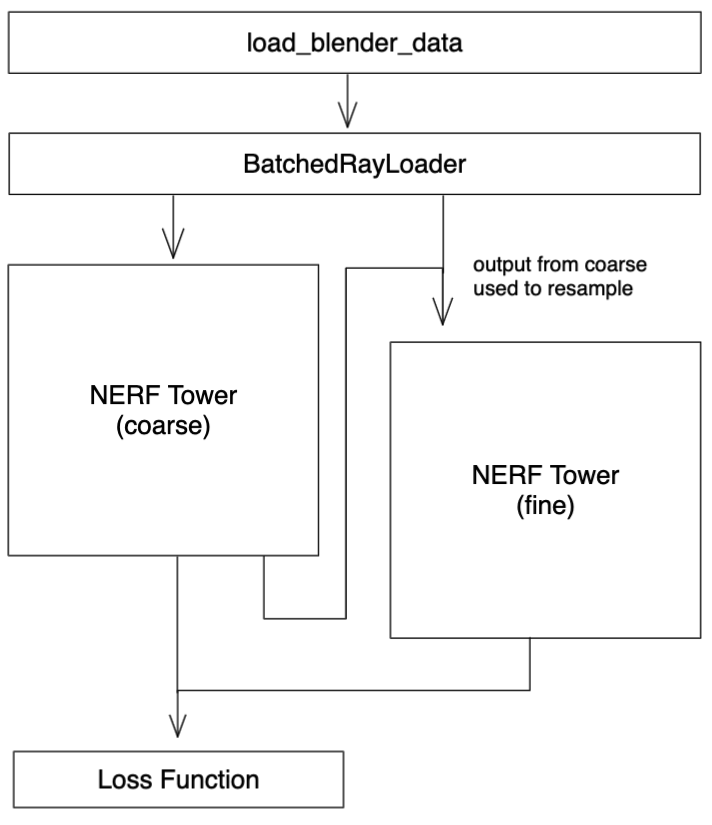
\includegraphics[width=80mm,scale=0.5]{images/train_arch.png}
    \caption{Hierarchical structure of the coarse and fine models.}
    \label{fine coarse}
\end{figure}



The logic of inverse transform sampling is largely as follows: we first create a cdf of the given distribution. Then we invert the cdf computationally by finding the value of x where the proportion of area to the left of x equals to a uniformly sampled point. This allows us to generate random samples from the probability distribution that is described by the output of the coarse network. Thus, in addition to having more points, the fine network has the additional benefit of having a stronger representation.

\subsubsection{Loss}

With two networks functioning simultaneously, our loss measures the MSE for both networks and add them (Eq.~\ref{Loss}). Here, $\mathfrak{R}$ is the set of rays in each batch, $C(r)$ is the ground truth rgb value of the pixels, $\hat{C_c}(r)$ is the coarse model's output, and $\hat{C_f}(r)$ is the fine model's output.

The loss includes the coarse model's output, even though it is not used directly to generate the final rendering output. This is because we would like to train the coarse network so that it can optimize in generating weights $w_i$ (Eq.~\ref{fine_sample}), which are used in sampling input points for the fine model.

\begin{equation}
\begin{aligned}
\mathcal{L} = \sum_{r \in \mathfrak{R}}  \biggr[\big\| \hat{C_c}(r) - C(r) \big\|_{2}^{2} + \big\| \hat{C_f}(r) - C(r) \big\|_{2}^{2} \biggr]
\end{aligned}
\label{Loss}
\end{equation}


\subsection{Model Structure Details}

\begin{figure}[h]
    \centering
    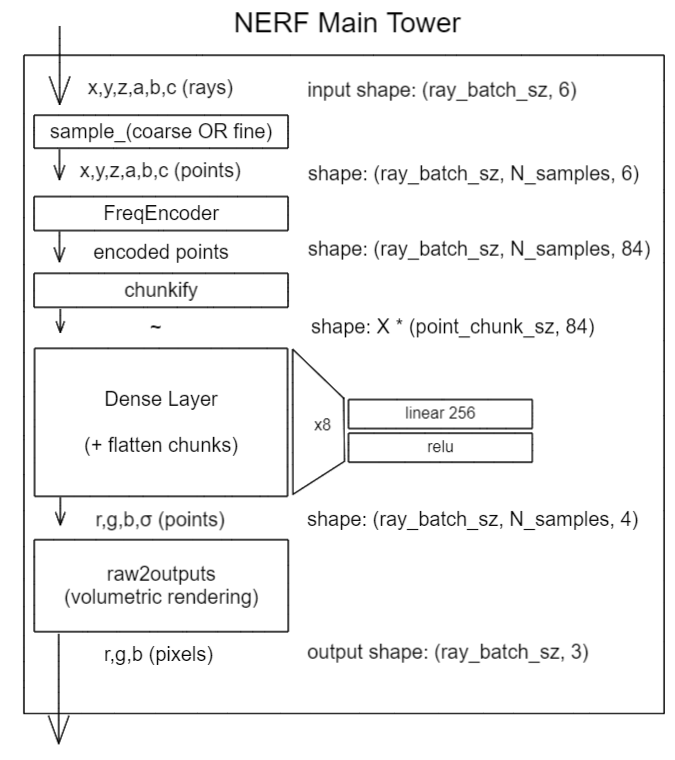
\includegraphics[width=80mm,scale=0.5]{images/nerf_arch_new.png}
    \caption{Model Structure Details.}
    \label{details}
\end{figure}
First, our data loader loads the training and testing images as a PyTorch Tensor. Then, our ray\_sampling function randomly samples an image from the training data, and 1024 pixels from the image, to generate 1024 rays corresponding to the pixels. Later, the fine (or coarse) sampling function samples points along the rays as input to the fine (or coarse) models, and the points are then embedded via the Frequency Encoder. We also chunkify the Tensor corresponding to the points into smaller chunks before feeding them into the model, relieving the GPU from processing too much information at the same time. Last, the model predicts the rgb values for the sampled pixels, and the loss is computed for back-propagation.



\section{Results}
Our model achieves a best peak signal-to-noise ratio (PSNR) of 31, which matches the average performance of the Realistic Synthetic 360{\textdegree} Dataset in the original paper (Table ~\ref{results}).

\begin{table} [h]
\begin{center}
\begin{tabular}{ l c c c }
\toprule
Object & Training Steps & Best Loss & Best PSNR \\
\midrule
Chair & 40k & 2.5e-3 & 31 \\
Ship &  160k & 4e-3 &  30 \\
Drums & 130k &8.5e-3 & 25.5 \\
Original Paper & up to 200k & N/A & Avg of 31 \\
\bottomrule
\end{tabular}
\end{center}
\caption{Training Results}
\label{results}
\end{table}
\begin{figure}[h]
    \centering
    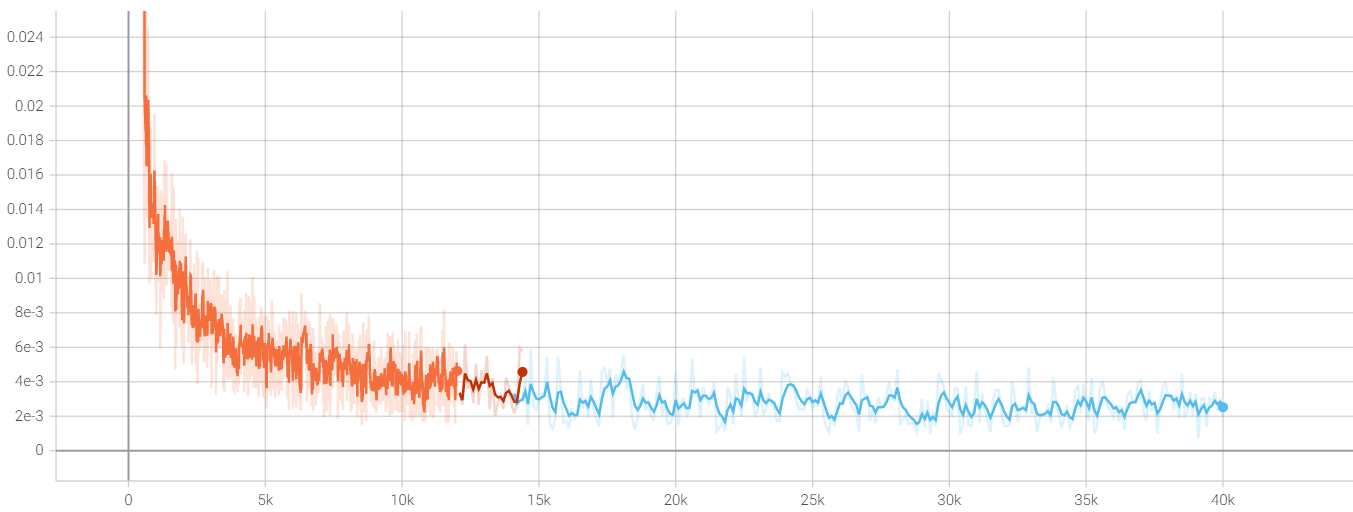
\includegraphics[width=80mm,scale=0.5]{images/chair_training_loss.png}
    Training loss.
    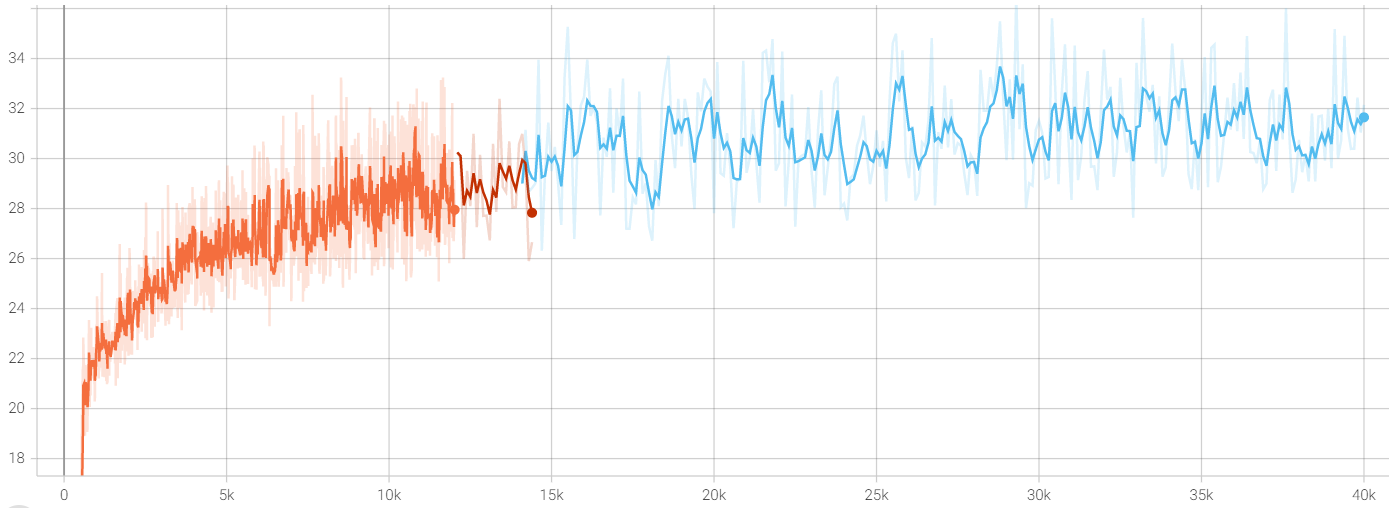
\includegraphics[width=80mm,scale=0.5]{images/chair_training_psnr.png}
    Training PSNR.
    \caption{Training for chair. The different colors indicate the model is trained in different sessions by saving and loading weights. \\ x axis: training step, each representing a batch of 1024 rays.}
    \label{train}
\end{figure}

\begin{figure}[h]
    \centering
    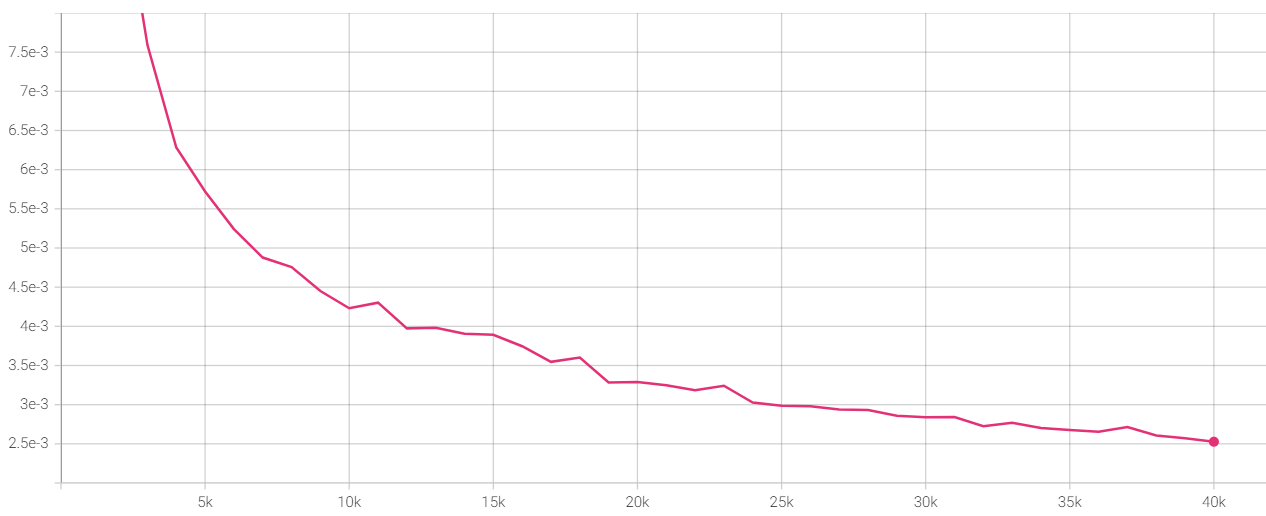
\includegraphics[width=80mm,scale=0.5]{images/chair_loss_tensorboard.png}
    Testing loss.
    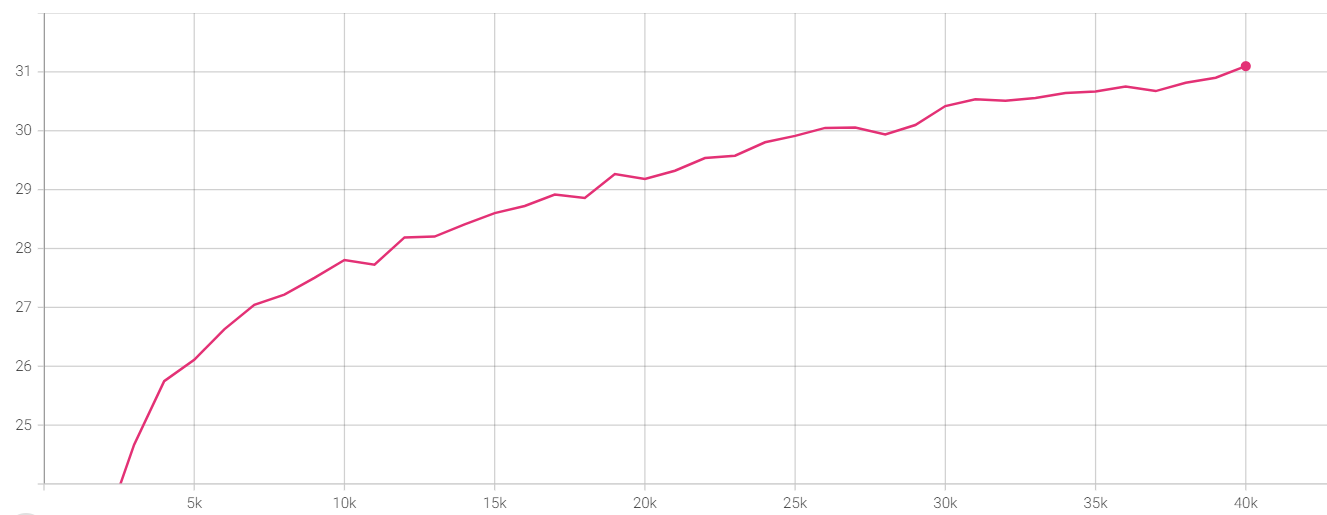
\includegraphics[width=80mm,scale=0.5]{images/chair_psnr_tensorboard.png}
    Testing PSNR.
    \caption{Testing for chair.\\ x axis: training step, each representing a batch of 1024 rays.}
    \label{test}
\end{figure}

Obviously, there is a large variance between each object (Table ~\ref{results}). As NeRF does not have transfer learning capabilities, it is purely object specific. The more complex objects (in terms of variety of colors, textures, transparency, and shadows) take much longer time to train.

\begin{figure}[h]
    \centering
    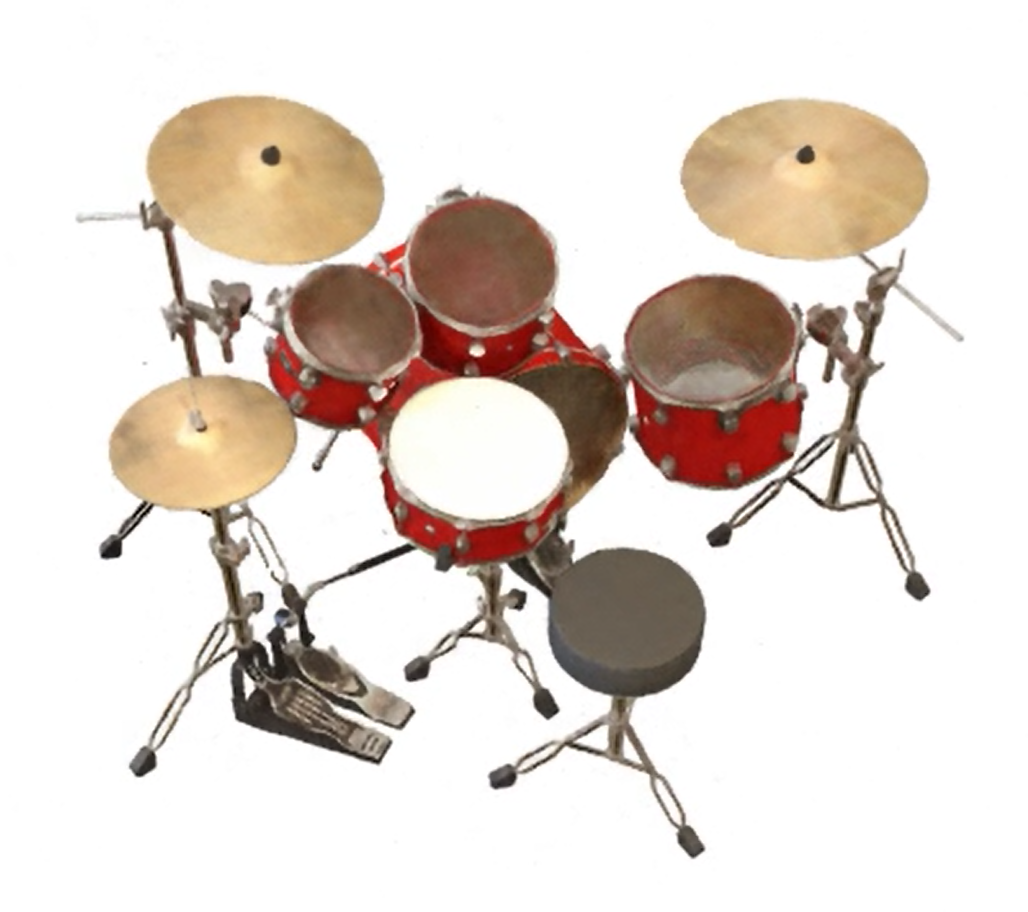
\includegraphics[width=40mm,scale=0.5]{images/drums.png}
    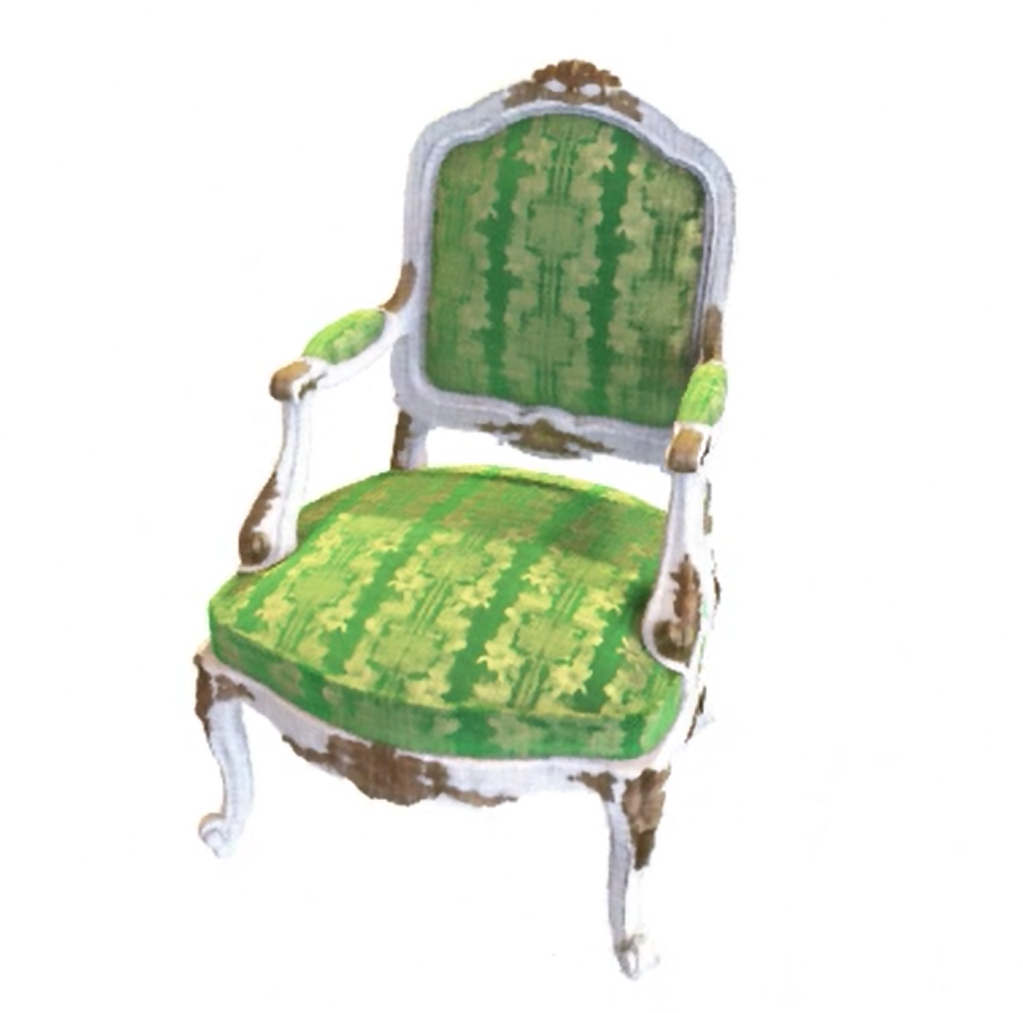
\includegraphics[width=40mm]{images/chair.png}
    \caption{The drums (left) have lots of reflective surfaces, making it harder to emulate the light reflection. The chair (right), on the other hand, converged much faster.}
    \label{ficus}
\end{figure}



In addition, we observed that during training, especially during the first thousand epochs (Fig ~\ref{train}), NeRFs are relatively unstable. This means that it may take a long time to confirm the state of training via loss curves. 

Having extremely long render times also does not help since this means that it is hard to evaluate the output image of a model intermittently during training. 

By comparing the training metrics (Fig ~\ref{train}) to the testing metrics (Fig ~\ref{test}), we also found that the training curve is much shakier than the lost curve. This may be due to the fact that for each training step, our model is given 1024 rays which correspond to 1024 pixels randomly sampled from one image of the training dataset. On the contrary, the testing is done by evaluating the model's performance on all 200 testing images, each containing $200 * 200$ pixels. In addition, we also found that the testing curves have relatively higher loss and lower PSNR compared to the training ones. Therefore, although each NeRF model is designated to perform on a fixed object (e.g., the synthesized chair), and the training images and testing images are both images of the same object, some overfitting problem does exist.

\section{Social Impact}

The implementation of the Neural Radiance Fields (NERF) paper could have huge social implications. For one, this technology could revolutionize the world of 3D graphics and virtual reality. It could change how we experience virtual reality and how we interact with it. It can democratize 3d modeling by reducing the barriers to entry by decreasing the need for industry know-how to create digital content.

However, there is also an increased risk of identity theft. Though this NERF implementation still requires camera pose information, it isn’t hard to imagine future developments estimating the camera poses as well. This will make it easier for malicious actors to take images from the internet and reconstruct 3d scans of objects, people and places.

Additionally, our experience confirmed the fact that NeRFs are very computationally intensive to train. Because the size of rays generated for each image, even with subsampling they require extremely long times to render for each epoch, meaning that both training as well as well as hyperparameter tuning require extremely large amounts of computing resources. This can have a large adverse effect on the environment should radiance fields take off as a mainstream method of rendering 3D objects.
%------------------------------------------------------------------------


%------------------------------------------------------------------------
\section{Conclusion}

The idea behind NeRF serves as a baseline moving forward for the application of deep learning in volumetric rendering, even models that do not use deep learning such as Plenoxels are directly inspired by NeRF. The hash embedding introduced in Instant NGP, which is a framework that work across multiple types of graphics applications, has one of the most potent applications in speeding up nerf. 

The results we achieved in this project prove that there is still a ton of potential for deep learning techniques in the fields of view synthesis and graphics. We hope that our work in this paper can help guide others who are interested in further expanding upon the NERF architecture or architectures inspired by it.

%------------------------------------------------------------------------



{\small
\bibliographystyle{plain}
\bibliography{ProjectFinal_ProjectReportTemplate}
}

%------------------------------------------------------------------------

\section*{Appendix}
\subsection*{Example Training and Output}


Here is the link to our outputs and weights: \href{https://drive.google.com/drive/folders/19VngwjdyA_Q5l2s-D8mha2ZMw6w8XV_c?usp=share_link}{nerf\_this\_outputs} 



\subsection*{Environment}
\begin{itemize}
    \item PyTorch 1.10 (and 1.13) with CUDA Toolkit 11.3
    \item GPU: RTX2060\textbackslash RTX3060\textbackslash M1 Ultra
\end{itemize}

\subsection*{Code}
Our codebase is divided into several files:
\begin{enumerate}
    \itemsep0em
    \item run.py contains the main function to run NeRF
    \item params.py contains all default params in an argumentparser
    \item batching.py contains the dataloader and data processing
    \item load\_blender.py contains the original code for reading raw data
    \item rays.py contains all ray helper functions and sampling used in render
    \item render.py contains batchified ray rendering
    \item model.py contains the MLP model
    \item encoding.py contains the frequency encoder
    \item raw2output contains a function that translates the raw model output into image rgb data
    \item validate.py contains the model validation function
    \item testing.py contains the model testing function for trained weights
    \item get\_device.py contains the helper function to check cuda or mps availability.
    \item generate\_output.py contains the function that renders output images and videos.
\end{enumerate}



\subsection*{TA meetings}
We met with out TA Anh Truong at Nov. 20 and Dec. 8.

\subsection*{Team contributions}

\begin{description}
\item [Andrew Ding] I worked on creating the main training loop, code for generating render output as well as intermittent JPEG outputs. I also wrote the batching.py logic for ray sampling. I also implemented the params.py for storing hyperparameters and certain training settings.
\item[Tony Zhu] I worked on ray batching, volumetric rendering, and all the supporting functions involved in sampling and rendering. I wrote the initial main function in run.py as well as the support code for testing and tensorboard logging. 
\item[Mingxuan Ji] I worked on the MLP model and its support functions. I also implemented the function (raw2outputs) which took in the outputs of the MLP model, and generated the rgb values of the corresponding pixels. Besides, I worked on the validation and model weights saving and loading.
\end{description}

\end{document}
